\chapter{Calibrated Drift Detection Method} \label{chapt:CDDM}

In this chapter we introduce calibrated drift detection method (CDDM), a drift detection method which detects increases in the irreducible error rate, rather than the overall error rate. Section \ref{CDDM:motivation} motivates the approach to concept drift detection taken by CDDM. Section \ref{CDDM:algorithm} provides the actual CDDM algorithm. Section \ref{CDDM:limitations} discusses theoretical and practical limitations of CDDM. Section \ref{CDDM:conclusion} summarises this chapter and discusses future work. 

%-------------------------------------------------------------------
% MOTIVATION
%-------------------------------------------------------------------

\section{Motivation} \label{CDDM:motivation}

Most, if not all, extant drift detectors assume that significant increases in the error rate of the base learner are due to concept drift and require model retraining. For example, Gama et al. \cite{DDM} state 
\begin{displayquote}
    Statistical [sic] theory \cite{statistical_theory} guarantees that while the class distribution of the examples is stationary, the error rate of the learning algorithm ($p_i$) will decrease when $i$ increases. A significant increase in the error of the algorithm, suggest a change in the class distribution, and that the actual decision model is not appropriate.
\end{displayquote}

\noindent However, this assumption is invalid in environments when 1) some labels can be predicted more easily than others, and 2) feature drift occurs. Consider the following (fictional) example from our motivating domain of medical triage:
\begin{displayquote}
    At a coronavirus emergency clinic, patients with coronavirus symptoms are being triaged. Young patients have a low mortality rate from coronavirus so are given low priority. Old patients have a high mortality rate so are given high priority. Middle aged patients, however, may have high or low mortality depending on other factors, so may be given a high, low, or medium priority. 
    
    The learner is easily able to discover the relationship between age and priority, but fails to make use of other features. The model thus has a higher error rate for middle aged patients than young or old patients. If there is an increase in the number of middle aged patients with corona virus, then the overall error rate of the model will increase.  
    
    A concept drift detector will may detect the increase in the error rate and signal that the model requires retraining. However, because the actual relationship between instances and labels has not changed, retraining the model would at best be a waste of time, and at worst result in an inferior model trained on a smaller dataset. 
\end{displayquote}
This example illustrates that what a concept drift detector should really be monitoring for is not increases in the overall error rate, but only increases in the error rate which can actually be reduced by retraianing. 

The average error rate (or {\it risk}) of the model is given by
\begin{align}
    R =& \Pr(\hat{y}=y) \\
    =& \int \Pr(\hat{y}\ne y|x)d\Pr(x).
\end{align}
A change in the risk can be thus be expressed
\begin{align}
	\Delta R =& \int \left( \Pr(\hat{y}\ne y|x) + \Delta \Pr(\hat{y}\ne y|x) \right) d\left( \Pr(x) + \Delta \Pr(x) .\right) \\
	 &- \int \Pr(\hat{y}\ne y|x)d\Pr(x). \\
	=& \int \Pr(\hat{y}\ne y|x) d\left(\Delta \Pr(x)\right) \\
	 &+ \int \Delta \Pr(\hat{y}\ne y|x) d\Pr(x) \\
	 &+ \int \Delta \Pr(\hat{y}\ne y|x) d\Delta \Pr(x)
\end{align}
Thus, the risk can be considered as the sum of three components. The {\bf change in irreducible error}, denoted
\begin{equation}
    \Delta R_I = \int \Pr(\hat{y}\ne y|x) d\Delta \Pr(x)
\end{equation}
is, the change in error rate due to changes in the instance distribution, rather than a change in the decision boundary. Because the decision boundary, has not changed, the increase in error rate cannot be counteracted by retraining the model. The {\bf change in reducible error}, denoted 
\begin{equation}
    \Delta R_I = \int \Delta \Pr(\hat{y}\ne y|x) d\Pr(x) \label{eq:re_err} 
\end{equation}
is error which {\it is} due to changes in the decision boundary and so can in principle be reduced by retraining the model. The final component
\begin{equation}
    - \int \Delta \Pr(\hat{y}\ne y|x) d\Delta \Pr(x)
\end{equation}
is an interaction term between changes in reducible and irreducible error. We will assume this is negligible for the rest of this discussion, so that
\begin{equation}
	\Delta R = \Delta R_I + \Delta R_R.
\end{equation}

Concept drift detection is typically operationalised as detecting an increase in the error rate of the model \cite{gama_survey}. Some drift detectors also monitor for declines in other metrics, such as precision and recall \cite{DDM-OCIa} or any changes in the confusion matrix \cite{LFR}, although for our purposes this makes no difference. Ideally, however, a drift detector should respond only to increases in the reducible error rate, and not the irreducible error rate. 

Detecting increases in the error rate rather than the reducible error rate can lead to two pathologies. The first is that feature drift may occur such that only irreducible error increases. 
\begin{align}
    \Delta R_R = 0, \quad \Delta R_I > 0 \quad \rightarrow \quad \Delta R > 0
\end{align}
This may trigger a drift detector, despite the fact that retraining will not be beneficial. Intuitively, this is a situation where the average difficulty of the prediction problems increases. Starting learning from scratch will not help, even though the error rate has increased.

The second is that feature drift may occur close to real drift, such that the reducible error rate increases, but the irreducible error rate decreases by at least as much. 
\begin{align}
    0 < \Delta R_R \le - \Delta R_I \quad \rightarrow \quad \Delta R \le 0
\end{align}
This results in a non-positive change in the overall error rate, so a drift detector will not be triggered when it should. Intuitively, this is a situation where the average difficulty of prediction problems {\it decreases}, but your ability to correctly answer the hard problems has decreased. It may pay to start learning from scratch, but because it looks like your performance is improving you don't consider the option.

Thus, in domains with non-homogeneous risk, and where feature drift may occur, we would like some way of detecting increases in the reducible error rate, rather than increases in the overall error rate. In the following section, we see how CDDM takes an initial step towards solving this problem.

%-------------------------------------------------------------------
% ALGORITHM
%-------------------------------------------------------------------

\section{Algorithm} \label{CDDM:algorithm}

Recall from the introduction that $q$ is the probability of a label given the instance, $\hat{q}$ is is the probability of a label given the instance, $\hat{q}$

CDDM approaches the problem of detecting increases in reducible error rather than overall error by estimating irreducible changes in the error rate, and subtracting this from the overall error rate:
\begin{equation}
	\Delta R_R = \Delta R - \Delta \hat{R_I}.
\end{equation}
This is achieved via an estimation of the residual:
\begin{align}
	\Delta R - \Delta \hat{R_I} =& \Delta \left( \Pr(\hat{y}\ne y) - \hat{\Pr}(\hat{y}\ne y) \right) \label{eq:cddm_tuna} \\
	=& \int \left( \Pr(\hat{y}\ne y|x) - \hat{\Pr}(\hat{y}\ne y|x) \right) d\left(\Delta \Pr(x)\right) \\
	 &+ \int \Delta \left( \Pr(\hat{y}\ne y|x) - \hat{\Pr}(\hat{y}\ne y|x) \right) d\Pr(x) \\
	=& \int \left( \Pr(\hat{y}\ne y|x) - \hat{\Pr}(\hat{y}\ne y|x) \right) d\left(\Delta \Pr(x)\right) \\
	 &+ \int \Delta \Pr(\hat{y}\ne y|x) d\Pr(x) \\
	 &- \int \Delta \hat{\Pr}(\hat{y}\ne y|x) d\Pr(x)
\end{align}
If the estimation is accurate then
\begin{equation}
	\Pr(\hat{y}\ne y|x) - \hat{\Pr}(\hat{y}\ne y|x) = 0.
\end{equation}
Additionally, a change in the error rate will not be immediately reflected as a change in the estimation of the error rate so 
\begin{equation}
	 \int \Delta \hat{\Pr}(\hat{y}\ne y|x) d\Pr(x) = 0.
\end{equation}
Thus, Equation \ref{eq:cddm_tuna} simplifies to
\begin{align}
	\Delta R - \Delta \hat{R_I} = \int \Delta \Pr(\hat{y}\ne y|x) d\Pr(x) = \Delta R_R.
\end{align}
Achieiving the dired result.

Intuitively, CDDM ``places bets" on how likely each predicted label is to be correct. If a prediction is estimated to have probability $p$ of being correct, then CDDM buys a bet for \$$p$. If the prediction turns out to be correct, CDDM receives a payoff of \$1. If the prediction turns out to be incorrect, CDDM receive a payoff of \$0. If CDDM loses a ``significant" amount of money, then it signals that concept drift has been detected.

Concretely, CDDM obtains residual estimations via calibrated probabilistic predictions. A predictor is {\bf calibrated} if it can assign probabilities to events which match the rates at which these events actually occur \cite{superforecasting}\cite{scoring_rules}\cite{calibrating}. For example, if a calibrated predictor assigns a probability of 90\% to ten events, then in expectation nine of those events should in fact obtain. 

Recall that we are denoting $q$ as the probability of a label obtaining a particular value, and $\qhatyhat$ a model's estimation of this value. Thus in our notation, a model is calibrated if $q=\hat{q}$. For the present, we will assume the label $y$ is binary, and so $q=\Pr(y=1)$. A plot of $q$ against $\hat{q}$ is known as a reliability diagram \cite{calibrating}. Figure \ref{fig:calibration} provides an illustration of the reliability diagram for a calibrated predictor.

\newcommand{\calibrationgraph}[7][]{
    % args:
    \draw [thick, <->] (0,1.25) -- (0,0) -- (1.25,0);
    \node [below] at (1.25,0) {$\hat{q}$};
    14
    \node [left] at (0,1.25) {$q$};
    \node [left] at (0,#7) {$\Pr(y_t=\hat{y}_t)$};
    \node [below] at (#6,0) {$\hat{q}_t$};
    \draw (#2,#3) -- (#4,#5);
    \draw [red] (#6,0) -- (#6,#7);
    \draw [red, dashed] (0,#7) -- (#6,#7);
}

\begin{figure}
    \centering
    \begin{tikzpicture}[scale=3]
        \calibrationgraph{0}{0}{1}{1}{0.5}{0.5}
    \end{tikzpicture}
    \caption{Calibration Graph}
    \label{fig:calibration}
\end{figure}

How are $\hat{q}$ values to be practically obtained? It is not possible to obtain $\hat{q}$ values for all machine learning techniques. Specifically, this cannot be done for any model which makes only point predictions, and not probabilistic probabilistic predictions. Decision trees are therefore excluded from this discussion. But most popular machine learning techniques produce outputs which can be interpreted as $\hat{q}$ values. For a neural network classifier, the activations of softmax or sigmoid units can be used as $\hat{q}$ values. For ensemble classifiers, the proportions of votes cast for a given label can be interpreted as $\hat{q}$. For a Bayesian model, the posterior probability is naturally interpreted as $\hat{q}$.

Assume we are dealing with a binary label. Let $\id{y=\hat{y}}=\id{y=0}$, $\qyhat=\Pr(y=0)$, and similarly for $\y{1}$, $\yhat{1}$, $\qhat{1}$, and so on (see Introduction for a full explication of notation). Additionally, let

\begin{align}
    \qyhat &= \Pr(y=\hat{y}) \\
    \qhatyhat &= \max(\qhat{0},\qhat{1})
\end{align}
These indicate the probability of the model making a correct prediction, and the models own estimation of this probability, respectively. 

CDDM takes as a null hypothesis that the base learner is calibrated. That is, the area in Equation \ref{eq:calibration_area} is equal to zero. In this case we have
\begin{align}
	\mathbb{E}\left[ \qhatyhat - \id{y=\hat{y}}  \right] &= \qyhat \cdot (\qhatyhat - 1) + (1-\qyhat) \cdot (\qhatyhat-0) \\
    &= \qyhat\qhatyhat - \qyhat + \qhatyhat - \qyhat\qhatyhat \\
    &= \qhatyhat - \qyhat.\label{eq:expectation}
\end{align}

Using this expected value, we can bound the probability of $\qhatyhat_t$ and $\id{y=\hat{y}}_t$ values to accumulating to a value as extreme as $k$ at time $T$
\begin{align}
    P\left(  \sum_{t=1}^T \frac{\qhatyhat_t - \id{y=\hat{y}}_t}{T} \ge k \right)
    &\le \exp\left(-\frac{2T^2k^2}{\sum_{t=1}^t(b_t - a_t)^2}\right) \\
    \intertext{Where $a_t$ and $b_t$ are lower and upper bounds on $\qhatyhat_t-\id{y=\hat{y}}_t$, respectively. Because $0\le \qhatyhat_t, \id{y=\hat{y}}_t\le 1$, we have that $a_t=-1 \le \qhatyhat_t-\id{y=\hat{y}}_t \le b_t=1$, so the right side of the inequality simplifies to}
  &\le \exp\left(-\frac{2T^2k_T^2}{\sum_{\tau=1}^t 4}\right) \\
  &\le \exp\left(-\frac{Tk_T^2}{2}\right). \label{eq:hoeffding}
\end{align}
This equation gives us a $p$-value of for an observed sequence of $\id{y=\hat{y}}$ and $\qhatyhat$ under the null hypothesis of calibration. If this value falls below some critical threshold, we may reject the null hypothesis and conclude that the model is uncalibrated. 

Similar to several other drift detectors \cite{DDM}\cite{HDDM}\cite{FLORA}, we use two critical thresholds: $\alpha_{warn}$, a warning threshold, and $\alpha_{drift}$, a drift threshold. When $P$ falls below $\alpha_{warn}$ for any $T$ value, CDDM issues a warning that drift may be occurring. When $P$ falls below $\alpha_{warn}$ for any $T$, CDDM signals that drift has been detected, and the referral documents since the earliest $T$ for which $P<\alpha_{warn}$ can be retrieved to retrain the model. We use the values $\alpha_{warn}=0.05$ and $\alpha_{drift}=0.01$.

Equation \ref{eq:hoeffding} indicates a trade-off in our choice of $T$, which in the streaming context denotes how large is the window of recent examples we are testing for miscalibration. The bound shrinks as $T$ and $k_T$ increase. However, if $T$ is large, then $k_T$, the mean value of $\qhatyhat-\id{y=\hat{y}}$ will be diluted by many pre-miscalibration instances. We do not have a principled way to choose a good value of $T$. Instead we propose maintaining a sliding window of $N$ values of $\qhatyhat-\id{y=\hat{y}}$, and testing the most recent $T$ instances for $T=1,2,\dots,N$. This introduces multiple comparisons and requires making a Bonferonni correction to our drift and warning bounds. The full pseudocode is given in Algorithm \ref{alg:cddm_basic}.

\begin{algorithm}
    \caption{CDDM}
    \label{alg:cddm_basic}
    \begin{algorithmic}
        \Require Warning threshold $\alpha_{warn}$
        \Require Drift threshold $\alpha_{drift}$
        \Require Window size $N$
        \State Window $\gets$ []
	\For {$y_t, \qyhat_t, \hat{y}_t$ in the data stream}
%            \State $\qhatyhat \gets \max(\qyhat,1-\qyhat)$
            \State Window.pop()
	    \State Window $\gets (\id{y=\hat{y}} - \qhatyhat) \cup$ Window
            \For {$T=1,2,\dots,N$}
                \State Calculate $p$ value for Window[:T]
                \If {$p \leq \alpha_{drift}/2N$}
                    \State {\tt status} $\gets$ {\tt drift}
                \ElsIf {$p_{min} \leq \alpha_{warn}/2N$}
                    \State {\tt status} $\gets$ {\tt warn}
                \EndIf
            \EndFor
        \EndFor
    \end{algorithmic}
\end{algorithm}

%-------------------------------------------------------------------
% LIMITATIONS
%-------------------------------------------------------------------

\section{Limitations} \label{CDDM:limitations}

\subsection{Theoretical Limitations}

There remains the possibility of miscalibration being undetectable by monitoring the area described in Equation \ref{eq:calibration_area} under certain conditions. One such condition is illustrated in Figure \ref{fig:weird_calibration}. It is not clear when such a situation could arise, and indeed if such a situation is even plausible. Further work is required to resolve this issue.

\begin{figure}
    \centering
    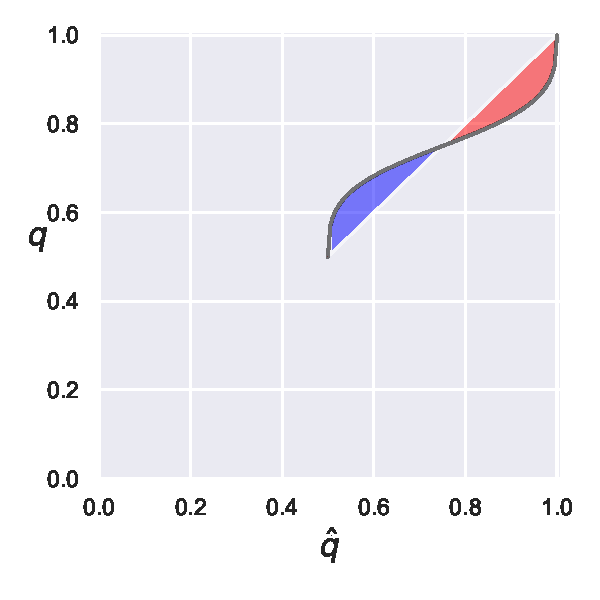
\includegraphics[width=0.5\textwidth]{images/cddm_area2.pdf}
    \caption{Example of a miscalibration undetectable by CDDM.}
    \label{fig:weird_calibration}
\end{figure}

We now consider the question of choosing an appropriate window size $N$. Given a window size $N$, our drift detection threshold will be given by $\epsilon/N$. Suppose also, that for the most recent $n$ examples we have had $\hat{q}-q=\delta$. That is, the model has become overconfident by $\delta$. Then the p-value will be given by
\begin{equation}
    \exp\left(-\frac{n^2\delta^2}{2N}\right)
\end{equation}
setting this equal to the threshold will give us the minimum time under the new distribution until the miscalibration can be detected. This gives
\begin{align}
    \exp\left(-\frac{n^2\delta^2}{2N}\right) &= \frac{\epsilon}{N} \\
    \delta &= \sqrt{-\frac{2N}{n^2}\ln\left(\frac{\epsilon}{N}\right)}
\end{align}
We get minimum $\delta$ when $n=N$. In this case, it takes the entire window to full up for the drift to be detected. Thus, the range of detectable $\delta$ given a window size $N$ is
\begin{equation}
    1 \ge \delta \ge \sqrt{-\frac{2}{N}\ln\left(\frac{\epsilon}{N}\right)} \label{eq:window_size}
\end{equation}

Figure \ref{fig:cddm_window_size} illustrates the minimum detectable $\delta$ against $N$ (black line), as well as the time to detect miscalibrations of $\delta$ values for a range of $N$ values (dashed lines).

\begin{figure}
    \centering
    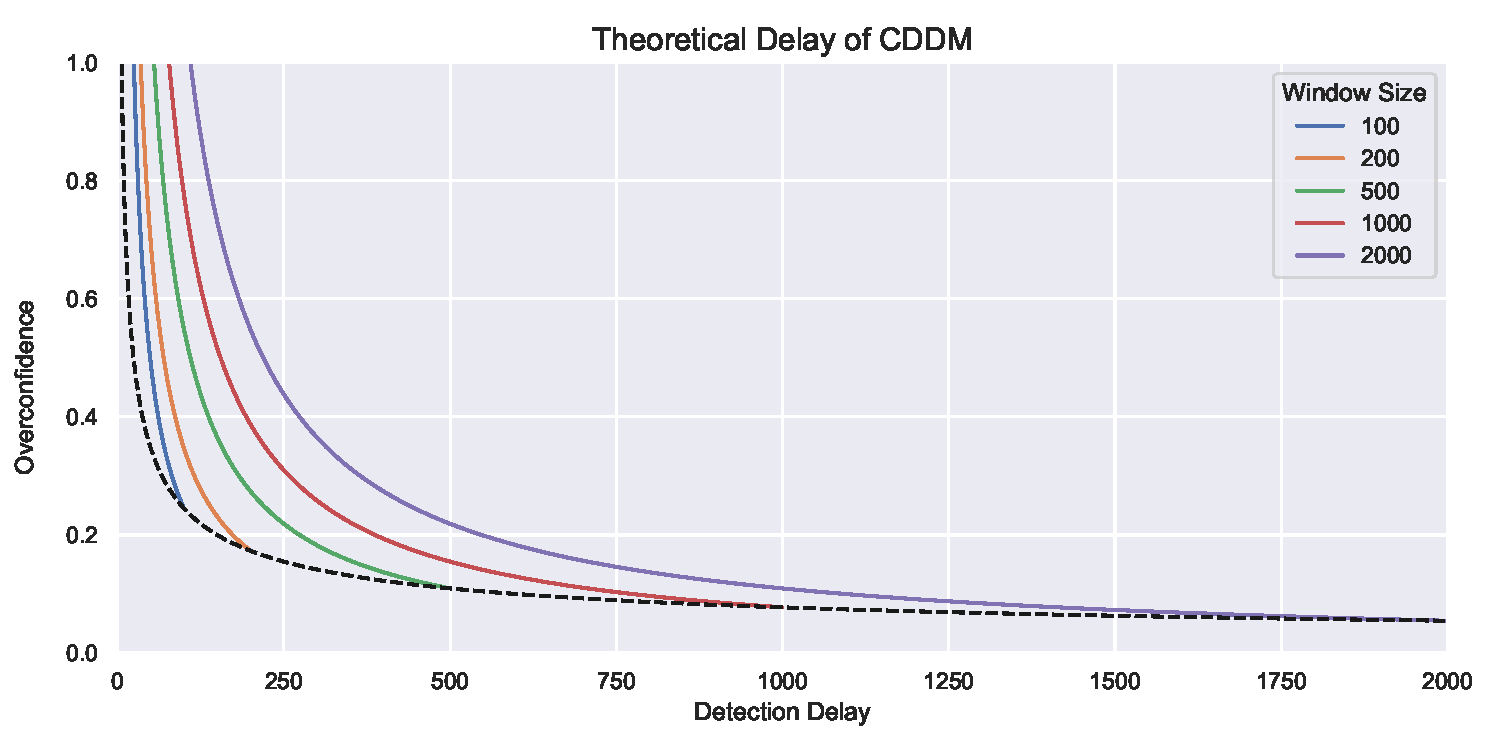
\includegraphics[width=\textwidth]{images/cddm_window_size.pdf}
    \caption{Detection delay (x-axis) vs $\delta$ (y-axis). The black line gives the minimum detectable $\delta$ for a window size $x$. The dashed lines are detection delays for window sizes of (from left to right) 100, 200, 500, 1000 and 2000.}
    \label{fig:cddm_window_size}
\end{figure}

An appropriate choice for window size $N$ can therefore be obtained by 1) if there is a smallest miscalibration degree $\delta$ which {\it requires} being detected, then one can obtain the appropriate window size using Equation \ref{eq:window_size}. 2) Otherwise, one may consult Figure \ref{fig:cddm_window_size}, and choose a window size which is appropriately reactive to miscalibration for the target domain.

%-------------------------------------------------------------------
% CALIBRATION
%-------------------------------------------------------------------

\subsection{Calibration}

CDDM assumes that a model starts out calibrated. In this section we consider strategies for ensuring that this is true.

\cite{nn_calibration}
\cite{trust_model_uncertainty}


For the purpose of discussing calibration, we will use the following terms to describe relationships between $q$ and $\hat{q}$.
\begin{itemize}
  \item If a predictor’s calibration map is the identity function, such that $q=\hat{q}$, then this predictor is {\bf well-calibrated}.
  \item If a predictor over-estimates the probabilities of a target outcome (in our case, a correct classification), and $\hat{q}>q$, then the model is {\bf overconfident}. Overconfident models can be considered as ``pushing" values towards 1 in the mapping from $q$ to $\hat{q}$.
  \item Conversely, if a predictor under-estimates the probabilities of a target outcome, and $\hat{q}<q$, then the predictor is {\bf underconfident}. Underconfident models can be considered as pushing $q$ values towards 0.
  \item If a predictor is overconfident close to 1 and underconfident close to 0, then the predictor is {\bf extremist}. Extremist models can be considered as pushing $q$ values towards 0 {\it and} 1. Maximum margin methods such as boosted trees and boosted stumps are prone to extremism \cite{calibrating}. Often an extremist predictor can be calibrated by applying a sigmoid-shaped map to subjective probabilities.
  \item The opposite type to extremisim is {\bf moderatism}, in which the predictor is underconfident close to 1 and overconfident close to 0. Thus, $q$ values are pushed {\it away from} 0 and 1. Na\"{i}ve Bayes models are prone to moderatism due to making unrealistic independence assumptions \cite{calibrating}. 
\end{itemize}
The terms ``overconfident" and ``underconfident" come from Tetlock \cite{superforecasting}. ``Extermism" and ``moderatism" are our own terminology. These relationships are illustrated with reliability diagrams in Figure \ref{fig:calib_drift_types}. Note that this list not exhaustive. Any function $f:[0,1]\rightarrow[0,1]$ is a possible relationship between $q$ and $\hat{q}$ for some model.

\begin{figure}%[t!]
    \centering
    \subfigure[Underconfident]{
        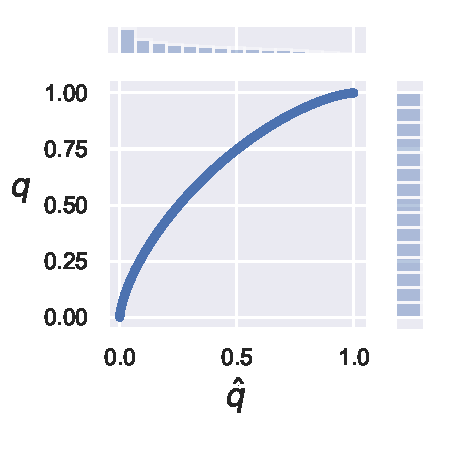
\includegraphics[width=0.45\textwidth]{images/overconfident.pdf}
    }
    \subfigure[Overconfident]{
        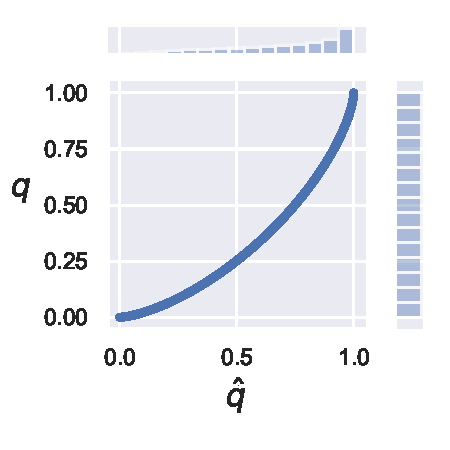
\includegraphics[width=0.45\textwidth]{images/underconfident.pdf}
    }
    \subfigure[Extremist]{
        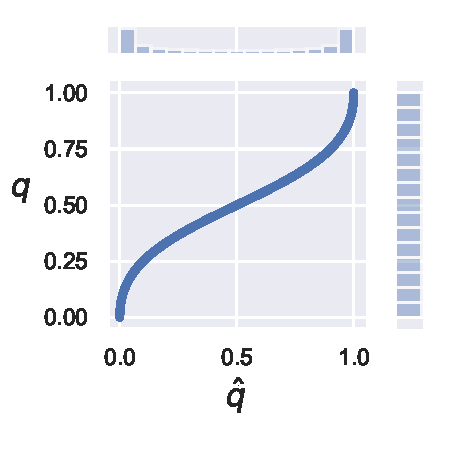
\includegraphics[width=0.45\textwidth]{images/extremist.pdf}
    }
    \subfigure[Moderate]{
        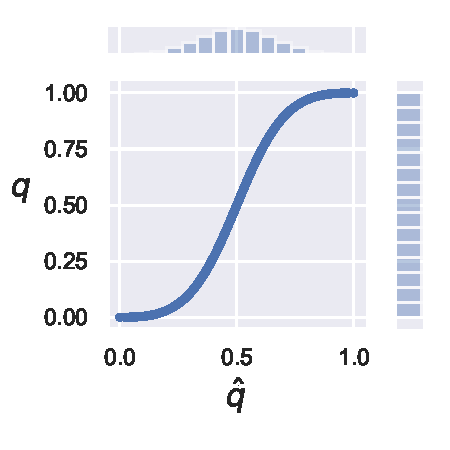
\includegraphics[width=0.45\textwidth]{images/moderate.pdf}
    }
    \caption{Reliability diagrams for a few relationships between $q$ and $\hat{q}$.}
    \label{fig:calib_drift_types}
\end{figure}

With the vocabulary of calibration and reliability diagrams, we may now return to our problem as laid out in Section \ref{CDDM:motivation}. We wished to derive an algorithm which could detect real drift {\it separately} from feature drift, as it it is only real drift which results in a change in the decision boundary. 

We identified two failure modes of only monitoring for increases in the error rate as a means of detecting concept drift. First, feature drift may trigger a drift detection, due to the average difficulty of the classification tasks increasing. Second, if feature drift and real drift co-occur, then the detector may fail to notice the concept drift due to the average difficulty of the classification tasks decreasing. 

These scenarios can be neatly expressed with reliability diagrams. Figure \ref{fig:no_drift} shows an initial distribution of data. The model is calibrated, and the $\hat{q}$ values centre around 0.5. These two facts together tell us that $\Pr(y=\hat{y})\approx 0.5$. 

Figure \ref{fig:co_drift} depicts the scenario in which real and feature drift co-occur, and the latter hides the former. A model in this situation would benefit from retraining, and yet a drift detector which is monitoring the error rate will not be triggered. Figure \ref{fig:pos_virt} depicts the scenario in which feature drift triggers will trigger a drift detector, despite no change in the decision boundary.

\newcommand{\calibrationgraphB}[7][]{
    % args:
    \draw [thick, <->] (0,1.25) -- (0,0) -- (1.25,0);
    \node [below] at (1.25,0) {$\hat{q}$};
    14
    \node [left] at (0,1.25) {$q$};
    \node [left] at (0,#7) {$\Pr(y=\hat{y})$};
    \node [below] at (#6,0) {$\mathbb{E}[\hat{q}]$};
    \draw (#2,#3) -- (#4,#5);
    \draw [red] (#6,0) -- (#6,#7);
    \draw [red, dashed] (0,#7) -- (#6,#7);
}

\newcommand{\virtualdriftgraph}[3][]{
    \begin{tikzpicture}[scale=3]
        \calibrationgraphB{0}{0}{1}{1}{0.5+#2}{0.5+#2}
        \draw [red, thick, ->] (0.5, #3) -- (0.5+#2*1.5, #3);
    \end{tikzpicture}
}

\begin{figure}
    \centering
    \begin{tikzpicture}[scale=3]
        \calibrationgraphB{0}{0}{1}{1}{0.5}{0.5}
    \end{tikzpicture}
        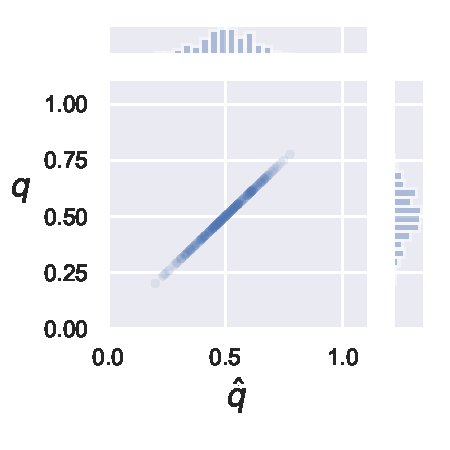
\includegraphics[width=0.3\textwidth]{images/no_drift.pdf}
    \caption{Original distribution.}
    \label{fig:no_drift}
\end{figure}

\begin{figure}
    \centering
    \begin{tikzpicture}[scale=3]
        \calibrationgraphB{0.25}{0}{1}{0.75}{0.75}{0.5}
        \draw [black, thick, ->] (0.9, 0.8) -- (0.9, 0.5);
        \draw [red, thick, ->] (0.6, 0.2) -- (0.85, 0.2);
    \end{tikzpicture}
        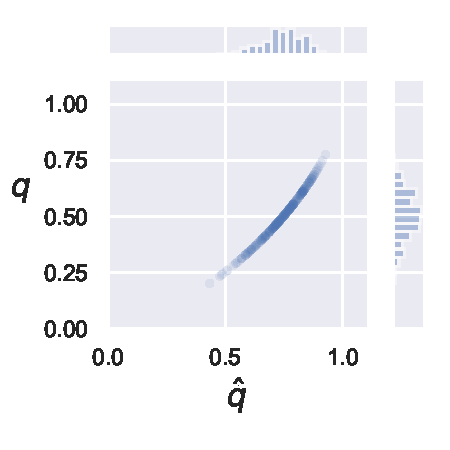
\includegraphics[width=0.3\textwidth]{images/hidden_drift.pdf}
    \caption{Virtual drift masking real drift.}
    \label{fig:co_drift}
\end{figure}

\begin{figure}
    \centering
    \virtualdriftgraph{-0.2}{0.125}     
    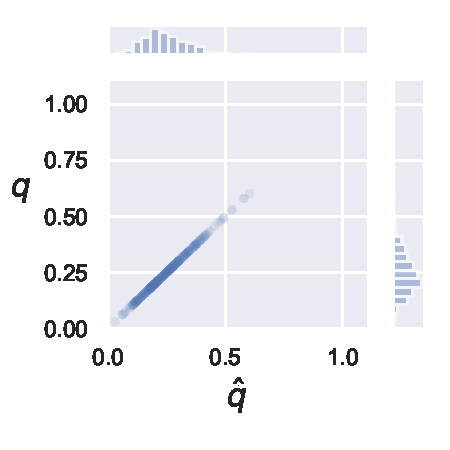
\includegraphics[width=0.3\textwidth]{images/positive_virtual.pdf}
    \label{fig:pos_virt}
    \caption{Negative drift decreasing the error rate.}
\end{figure}

What we have shown by these examples is that concept drift detectors should not be monitoring for changes in the error rate, as this influenced by feature drift, and will lead to impaired performance. Instead, we should be monitoring for changes in the reliability diagram of a model. This is the true test for whether real drift has occurred, regardless of what feature drift may or may not be occurring.

\subsection{Scoring Rules}

We begin with the easiest case in which calibration can be achieved: the degenerate case in which models are already calibrated. The most common way to arrive at a model which is calibrated, is to train it to minimise a loss function with certain properties. 

Let $P$ be a probability measure over some outcome space $\Omega$, denoting the subjective probabilities assigned by the predictor. $\omega \in \Omega$ denotes the actual outcome. The predictor’s loss for this prediction is given by a {\bf scoring rule} of the form $S(P,\omega)$. Let $Q$ be the true probability distribution over $\Omega$, then
\begin{equation}
	S(P,Q) = \int_x S(P,x)Q(x) 
\end{equation}
Is the expected score of a subjective probability $P$. A scoring rule is {\bf proper} if 
\begin{equation}
	S(Q,Q) \ge S(P,Q)
\end{equation}
for all $P,Q$. That is, no higher score can be achieved than by predicting the true probability distribution. In other words, if you know the true probability distribution, you cannot ``game” the scoring rule and achieve a higher score by guessing something different from the true distribution. A scoring rule is {\bf strictly proper} if
\begin{equation}
	S(Q,Q) > S(P,Q)
\end{equation}
for all $P,Q$. That is, the {\it only} way to achieve the highest score is by guessing the true probability distribution.

If a proper scoring rule is used as a model’s loss function, and a model is sensibly trained to minimise this loss function, such as with gradient descent, hyperparameter selection on a development set, and early stopping, then the model should end up well calibrated. We now discuss some examples of proper scoring rules, noting if and when these rules are used in machine learning.

One of the most famous scoring rules is the {\bf quadratic scoring rule}, which is strictly proper and has the form
\begin{equation}
	S(P,\omega) = 2 P_\omega - P \dot P = 2 P_\omega - \sum_i P_i^2
\end{equation}
An affine transformation of this rule yields the equivalent but more elegant Brier scoring rule \cite{scoring_rules}
\begin{equation}
	S(P,\omega) = \sum_i (y_i - P_i)^2
\end{equation}
where $y_i = \mathds{1}[\omega=i]$. Brier scoring is equivalent to mean square errors, which are used as loss functions in many machine learning contexts, although usually for regression problems rather than classification problems.

Another famous scoring rule is the {\bf logarithmic scoring rule}, which is also strictly proper and takes the form
\begin{equation}
	S(P,\omega) = \log (p_\omega)
\end{equation}
For binary and categorical predictions, this is equivalent to {\bf categorical cross entropy} which is a very common loss function in deep learning, in which it is more commonly expressed
\begin{equation}
	S(P,\omega) = \sum_i y_i \log(p_i)
\end{equation}
where $y_i = \mathds{1}[\omega=i]$ again. Thus a deep learning model with this loss function which has been sensibly trained should be well calibrated.

Another common scoring rule which is strictly proper is {\bf spherical scoring} which takes the form
\begin{equation}
	S(P,\omega) = \frac{P_\omega}{\|P\|}.
\end{equation}
Spherical scoring does not have particular relevance to machine learning.

\subsection{Calibration Maps}



If a model was not trained using a proper scoring rule, or for some other reason is not well calibrated, then it can become approximately well-calibrated using a {\bf calibration map}. There are several approaches to producing calibration maps, described below.

\subsubsection{Logistic Calibration}

Logistic calibration - also called {\bf Platt scaling} \cite{platt} - calibrates model predictions by passing them through a parametric calibration map, specifically a sigmoid function. If $\bar{p}$ is the (uncalibrated) model output, then a calibrated probability is given by
\begin{equation}
	p = \frac{1}{1 + \exp(a\bar{p} + b)}
\end{equation}
where the parameters a and b are fitted using maximum likelihood estimation on a calibration set $(p_1,L_1),\dots,(p_n,L_n)$. Note that this calibration set must be distinct from the training set, but can be the same set as used for (hyper)parameter selection. Specifically, $a$ and $b$ are derived from performing gradient descent on the loss function
\begin{equation}
	- \sum_i L_i \log( p_i ) + (1-L_i) \log(1-p_i)
\end{equation}
To avoid overfitting, Platt recommends modifying the loss values before fitting the sigmoid calibration map as follows:
\begin{equation}
	L_i' = \begin{cases}
		\frac{N_1 + 1}{N_1 + 2} & \text{if }L_i=1 \\
		\frac{1}{N_0 + 2} & \text{if }L_i=0 \\
	\end{cases}
\end{equation} 
where $N_0$ is the number of zero-valued losses, and $N_1$ is the number of one-valued losses. 

% \subsubsection Isotonic Calibration}
% 
% Isotonic calibration is a non-parametric method of producing calibration maps (cite Zadrozny and Elkan 2002; 2001, Robertson et al., 1988). It follows that it is more flexible than logistic calibration, but also more prone to overfitting. The only assumption isotonic regression makes about the reliability diagram is that it is isotonic, that is, it is monotonically increasing. The pair-adjacent ventilators algorithm (PAV) algorithm is one approach to finding such an isotonic map, as given below (Cite Ayer et al., 1955). TODO: explain PAV.

\subsubsection{Beta Calibration}

Beta calibration is another parametric calibration map family \cite{beyond_sigmoids}. It takes the form
\begin{equation}
	p = \frac{1}{1 + 1/\left(e^c\frac{\hat{p}^a}{(1-\hat{p})^b}\right) }
\end{equation}
where $a,b\ge 0$ so that the map is monotonically non-decreasing. This map can be fitted as easily as a logistic map \cite{beyond_sigmoids}.

Beta calibration is intended to overcome some of the drawbacks of logistic calibration. Logistic calibration results in distortions for many classifiers including Naive Bayes and Adaboost which can result in worse probability estimates than the original. The  strength of logistic calibration is that it tends towards producing exactly correct calibration when a model's uncalibrated probabilities are normally distributed. Beta calibration, on the other hand, tends towards correct calibration when the uncalibrated probabilities are beta distributed.

Experiments have found beta calibration to be superior to logistic calibration for Na\"{i}ve Bayes, Adaboost, Random Forest, logistic regression, SVM, and MLP \cite{beyond_sigmoids}. 

%-------------------------------------------------------------------
% CONCLUSION
%-------------------------------------------------------------------

\section{Conclusion} \label{CDDM:conclusion}

In this chapter we introduced calibrated drift detection method (CDDM). We argued that a drift detector should detect increases in the reducible error rate rather than the overall error rate, so as to avoid unnecessary retraining. CDDM takes this approach to concept drift detection by detecting when a model becomes uncalibrated. However, CDDM still has some significant limitations. Theoretically, CDDM can only detect mean overconfidence below a certain level determined by the window length. Practically, CDDM assumes that a learner is initially calibrated, whereas most models are not natively calibrated and post-hoc calibration techniques have significant limitations.

A promising direction for future work would be building a calibration map online, and detecting when this calibration map changes, rather than assuming the learner is calibrated in the first place.